\begin{minipage}[t]{0.49\linewidth}\centering
{\color{black}\normalsize\bfseries LLM + RAG}\par\smallskip
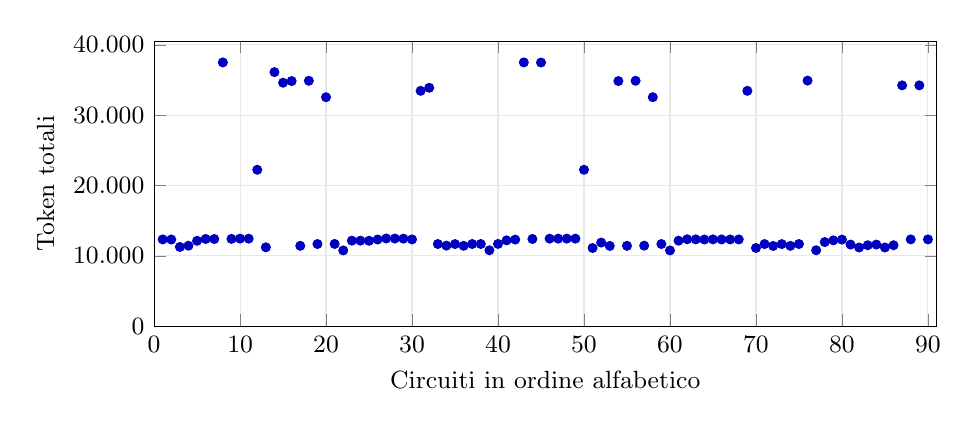
\begin{tikzpicture}\begin{axis}[width=0.95\linewidth,height=5.2cm,grid=major,grid style={gray!18},tick label style={font=\small},label style={font=\small},scaled ticks=false,/pgf/number format/use comma,unbounded coords=discard,xlabel={Circuiti in ordine alfabetico},ylabel={Token totali},xmin=0,xmax=91,ymin=0,ymax=40515.12,]
\addplot[color=blue!75!black,mark=*,mark size=1.6pt,only marks] coordinates {(1,12344) (2,12331) (3,11271) (4,11450) (5,12150) (6,12407) (7,12401) (8,37514) (9,12419) (10,12457) (11,12450) (12,22248) (13,11222) (14,36131) (15,34623) (16,34862) (17,11430) (18,34903) (19,11688) (20,32566) (21,11701) (22,10779) (23,12165) (24,12167) (25,12152) (26,12329) (27,12477) (28,12468) (29,12454) (30,12344) (31,33472) (32,33904) (33,11691) (34,11460) (35,11681) (36,11432) (37,11690) (38,11690) (39,10800) (40,11703) (41,12209) (42,12319) (43,37513) (44,12407) (45,37496) (46,12454) (47,12454) (48,12457) (49,12450) (50,22248) (51,11124) (52,11896) (53,11417) (54,34862) (55,11430) (56,34903) (57,11458) (58,32566) (59,11687) (60,10779) (61,12165) (62,12365) (63,12350) (64,12329) (65,12352) (66,12341) (67,12341) (68,12344) (69,33472) (70,11126) (71,11685) (72,11416) (73,11681) (74,11432) (75,11690) (76,34929) (77,10800) (78,11968) (79,12209) (80,12317) (81,11612) (82,11195) (83,11517) (84,11612) (85,11195) (86,11517) (87,34249) (88,12347) (89,34249) (90,12347)};
\end{axis}\end{tikzpicture}
\end{minipage}
\hfill\begin{minipage}[t]{0.49\linewidth}\centering
{\color{black}\normalsize\bfseries LLM no RAG}\par\smallskip
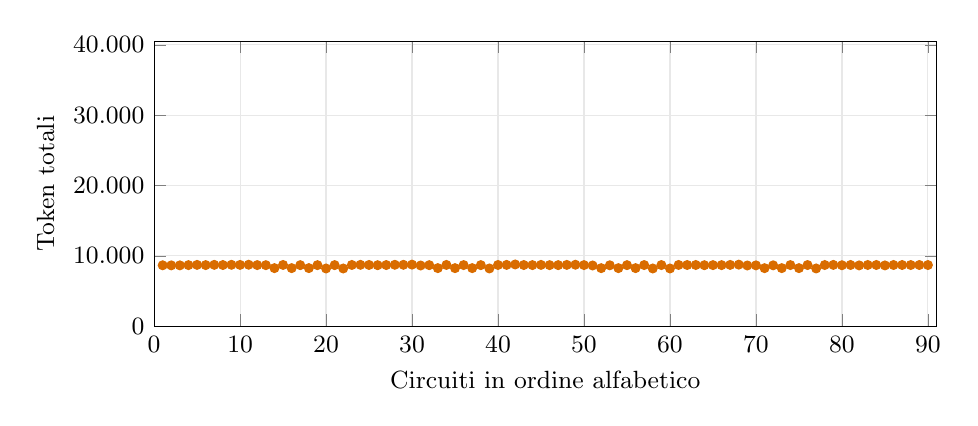
\begin{tikzpicture}\begin{axis}[width=0.95\linewidth,height=5.2cm,grid=major,grid style={gray!18},tick label style={font=\small},label style={font=\small},scaled ticks=false,/pgf/number format/use comma,unbounded coords=discard,xlabel={Circuiti in ordine alfabetico},ylabel={Token totali},xmin=0,xmax=91,ymin=0,ymax=40515.12,]
\addplot[color=orange!85!black,mark=*,mark size=1.6pt,only marks] coordinates {(1,8667) (2,8655) (3,8654) (4,8691) (5,8723) (6,8693) (7,8729) (8,8705) (9,8733) (10,8720) (11,8744) (12,8694) (13,8682) (14,8261) (15,8713) (16,8261) (17,8685) (18,8264) (19,8685) (20,8212) (21,8691) (22,8212) (23,8712) (24,8730) (25,8711) (26,8678) (27,8700) (28,8736) (29,8734) (30,8758) (31,8637) (32,8684) (33,8263) (34,8715) (35,8261) (36,8696) (37,8262) (38,8688) (39,8214) (40,8709) (41,8720) (42,8783) (43,8703) (44,8693) (45,8721) (46,8687) (47,8688) (48,8720) (49,8744) (50,8694) (51,8638) (52,8259) (53,8665) (54,8261) (55,8685) (56,8264) (57,8698) (58,8212) (59,8699) (60,8212) (61,8712) (62,8706) (63,8707) (64,8678) (65,8690) (66,8689) (67,8719) (68,8758) (69,8637) (70,8655) (71,8257) (72,8660) (73,8261) (74,8696) (75,8262) (76,8700) (77,8214) (78,8703) (79,8720) (80,8674) (81,8709) (82,8649) (83,8708) (84,8709) (85,8649) (86,8708) (87,8706) (88,8702) (89,8706) (90,8702)};
\end{axis}\end{tikzpicture}
\end{minipage}
\par\vspace{0.25cm}\begin{minipage}[t]{0.49\linewidth}\centering
{\color{black}\normalsize\bfseries MQT Predictor}\par\smallskip
\parbox[c][5.2cm][c]{\linewidth}{\centering\large Non applicabile\\[5pt]\normalsize Questo sistema non usa un LLM.}
\end{minipage}
\hfill\begin{minipage}[t]{0.49\linewidth}\centering
{\color{black}\normalsize\bfseries Random}\par\smallskip
\parbox[c][5.2cm][c]{\linewidth}{\centering\large Non applicabile\\[5pt]\normalsize Questo sistema non usa un LLM.}
\end{minipage}
\par\vspace{0.25cm}\makebox[\linewidth][c]{%
\begin{minipage}[t]{0.49\linewidth}\centering
{\color{black}\normalsize\bfseries LLM + Random RAG}\par\smallskip
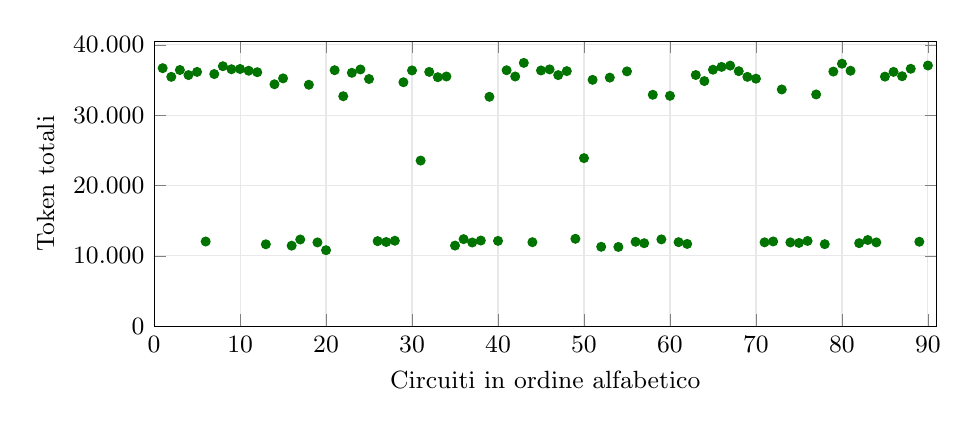
\begin{tikzpicture}\begin{axis}[width=0.95\linewidth,height=5.2cm,grid=major,grid style={gray!18},tick label style={font=\small},label style={font=\small},scaled ticks=false,/pgf/number format/use comma,unbounded coords=discard,xlabel={Circuiti in ordine alfabetico},ylabel={Token totali},xmin=0,xmax=91,ymin=0,ymax=40515.12,]
\addplot[color=green!45!black,mark=*,mark size=1.6pt,only marks] coordinates {(1,36694) (2,35463) (3,36435) (4,35713) (5,36162) (6,12046) (7,35859) (8,36971) (9,36542) (10,36579) (11,36329) (12,36119) (13,11651) (14,34406) (15,35242) (16,11455) (17,12332) (18,34337) (19,11918) (20,10810) (21,36405) (22,32704) (23,36034) (24,36510) (25,35153) (26,12102) (27,11975) (28,12154) (29,34695) (30,36373) (31,23556) (32,36163) (33,35411) (34,35510) (35,11469) (36,12382) (37,11908) (38,12184) (39,32626) (40,12136) (41,36399) (42,35513) (43,37446) (44,11949) (45,36368) (46,36521) (47,35708) (48,36276) (49,12433) (50,23903) (51,35034) (52,11296) (53,35350) (54,11275) (55,36239) (56,12005) (57,11803) (58,32912) (59,12349) (60,32762) (61,11956) (62,11702) (63,35722) (64,34858) (65,36476) (66,36875) (67,37057) (68,36267) (69,35460) (70,35199) (71,11930) (72,12055) (73,33667) (74,11919) (75,11840) (76,12126) (77,32958) (78,11668) (79,36210) (80,37328) (81,36326) (82,11810) (83,12261) (84,11921) (85,35495) (86,36163) (87,35547) (88,36608) (89,12012) (90,37073)};
\end{axis}\end{tikzpicture}
\end{minipage}
}\par
